\utilchap{dem2fds - A utility for creating FDS an input file from digital elevation map (dem) data}

This \textchap\ gives notes on creating FDS input files from digital elevation map (dem) files using the utility dem2fds.
dem2fds is a utility installed along with FDS and Smokeview that may be used to convert elevation and image data obtained
from the USGS website \hhref{https://viewer.nationalmap.gov/basic} into FDS input files.

\utilsect{Preliminaries}

\begin{itemize}
\item Download and install Smokeview from \hhref{https://pages.nist.gov/fds-smv/downloads.html}.
This download provides the utility dem2fds used for creating FDS input files.

\item Download and install Imagemagick from \\  \hhref{http://www.imagemagick.org/script/binary-releases.php}.
This program is used to convert terrain images files from jpeg 2000 to jpeg format.

\item Go to the USGS National Map website at \hhref{https://viewer.nationalmap.gov/basic} to obtain elevation and terrain image data files
for the region of interest.
These files are used by dem2fds to create FDS input files.
This website has a map of the United States on the right and a set of data download options is on the left.
Zoom in on the region of interest then download elevation ( Elevation Products (3DEP) ) and terrain image ( Imagery - 1 meter (NAIP) ) files using the steps described below.

\begin{figure}[bph]
\centerline{
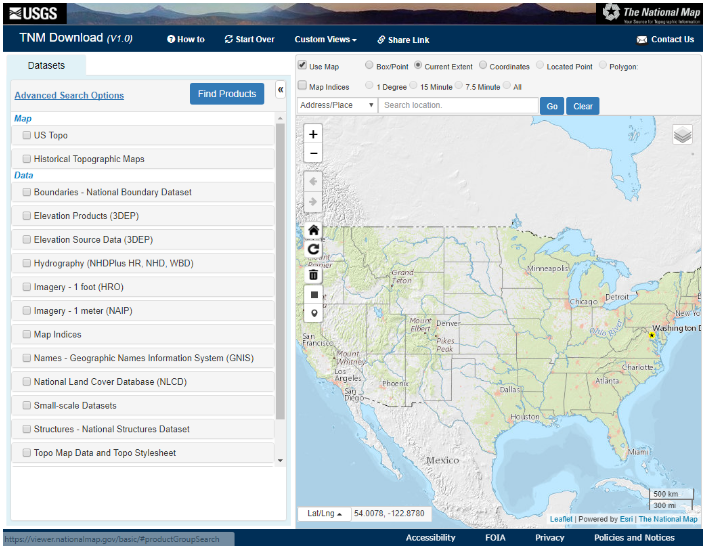
\includegraphics[width=4.5in]{FIGURES/usgsdem}}
 \caption[FDS file overview]{USGS website for obtaining digital elevation map data and terrain images}
\label{usgswebsite}%
\end{figure}

\begin{itemize}
\item Obtain Elevation data

\begin{enumerate}
\item Select the {\em Elevation Products (3DEP)}\ checkbox.
\item Select 1/3 arc-second DEM checkbox
\item Select the {\em GridFloat}\ File format option
\item Click on the map and zoom in to a region of interest.
\item Click on the {\em Find Products}\ button.  You should see one or more
entries listed with headings beginning with
USGS NED 1/3 arc-second ...... 1 x 1 degree .
\item Click on the {\em Footprint}\ link to verify where various files are located.
\item Click on {\em Download}\ link to download files of interest.
\item Unzip these files using a program such as Winzip. Open the directory created with the unzip operation and
copy the .flt and .hdr files to a directory where you'll keep your elevation and image files.
\end{enumerate}

\item Obtain Terrain Images
\begin{enumerate}
\item Click on the {\em Return to Search}\ button
and uncheck (if checked) the {\em Elevation Products (3DEP)}\ checkbox
\item Select the {\em Imagery - 1 meter (NAIP)}\ checkbox
\item Click on the map and zoom in to
a region of interest within the elevation region selected for elevation files.
\item Click on the {\em Find Products}\ button.  You should see one or more
entries with each entry beginning with {\tt m\_}\ and ending with {\tt .jp2} .
\item Click on the {\em Footprint}\ link to verify image file locations.
\item Click on {\em Download}\ link to download files of interest. The image files should
cover the region you are using to define an FDS input file.
\item Copy the downloaded files to the same directory you used to copy the .flt and .hdr elevation files.
\item The .jp2 files you just downloaded are in {\em jpeg 2000}\ format.
They need to be converted to jpeg format .
To do this on a PC, run the {\tt jp2conv}\ command.
On Linux or a Mac, run the {\tt jp2conv.sh}\ command.
These commands are installed with the latest version of Smokeview.
\end{enumerate}
\end{itemize}
\end{itemize}

\utilsect{Creating an FDS input file from dem data}
\begin{itemize}
\item Create a dem2fds input file.

Create a file named {\tt casename.in}\ containing the following lines

\begin{verbatim}
GRID
  ibar jbar kbar
LONGLATMINMAX
  longmin  longmax latmin latmax
\end{verbatim}

where {\tt ibar}\ and {\tt jbar}\ are the number of longitude and latitude divisions
and {\tt kbar}\ is the number of divisions along the z direction and
{\tt longmin}, {\tt longmax}, {\tt latmin}\ and {\tt latmax}\
are the minimum and maximum
longitude and latitude of the region  being modeled.

Two other methods for specifying a terrain region are to use the
{\tt LONGLATCENTER}\ or {\tt LONGLATORIG}\ keywords as in

\begin{verbatim}
GRID
  ibar jbar kbar dx dy
LONGLATCENTER
  longcen  latcen
\end{verbatim}

or

\begin{verbatim}
GRID
  ibar jbar kbar dx dy
LONGLATORIG
  longorig  latorig
\end{verbatim}

where {\tt dx}\ and {\tt dy}\ are the scenario width and length in meters
( {\tt ibar}, {\tt jbar}\ and {\tt ibar}\ are defined as before),
{\tt longcen}\ and {\tt latcen}\ are the longitude and
latitude at the scenario center,
{\tt i.e.}\ at position ({\tt dx/2}, {\tt dy/2})
and {\tt longorig}\ and {\tt latorig}\ are the longitude and
latitude at the scenario origin,
{\tt i.e.}\ at position ({\tt 0.0, 0.0}).

\item To create an FDS input file, run the command:
\begin{verbatim}
 dem2fds -d elevation_directory casename.in
\end{verbatim}
where {\tt elevation\_directory}\ is the path of the directory containing the
elevation and image files downloaded previously and
casename.in is the file containing {\tt GRID}\ and {\tt LATLONG...}\ keywords.

\item To view the case, run the commands:
\begin{verbatim}
fds casename.fds
smokeview casename
\end{verbatim}
\end{itemize}

Note, the FDS input file, {\tt casename.fds}\ is only a starting point.  You will need to
edit it to model your scenario as you wish.

\utilsect{Overview of dem2fds Input Keywords}

\blist
\hitem{GRID} Specifying the simulation grid
\begin{verbatim}
GRID
 ibar jbar kbar dx dy zmin zmax
\end{verbatim}

ibar, jbar, bar - number of divisions along the x, y and z directions
dx, dy - distance along the x and y axis.

Note, dx and dy are required if LATLONGCENTER or
LATLONGORIG are used to specify a terrain region and
optional if LATLONGMINMAX is used to specify a terrain region (dem2fds computes
dx and dy for LATLONGMINMAX keywords).

zmin, zmax - minimum and maximum z elevation.  These parameters are optional.


\hitem{LONGLATCENTER} - specifying the longitude and latitude at the scenario center

\begin{verbatim}
LONGLATCENTER
 longcen latcen
\end{verbatim}


longcen, latcen - longitude and latitude at the center of the scenario, at
position (dx/2,dy/2) .

\hitem{LONGLATORIG}- specifying the longitude and latitude at the scenario origin
\begin{verbatim}
LONGLATORIG
 longorig latorig
\end{verbatim}


longorig, latorig - longitude and latitude at the origin of the scenario, at
position (0,0) .

\hitem{LONGLATMINMAX} - specifying longitudes and latitudes that bound the scenario
\begin{verbatim}
LONGLATMINMAX
 longmin longmax latmin latmax
\end{verbatim}


longmin, longmax - minimum and maximum longitude
latmin, latmax - minimum and maximum latitude

\elist

\utilsect{dem2fds Command Line Options}

\lstinputlisting{SCRIPT_FIGURES/dem2fds.help}

\begin{enumerate}
\item The {\tt -obst}\ option is used by default.
\item The {\tt -geom}\ option is experimental testing the new geometry file format.
\item All terrain images should contain a 300 pixel overlap buffer.  However
this is not always the case.  The {\tt -nobuffer}\ option is used for those
cases when there is no overlap between two adjacent images.
\end{enumerate}

\utilsect{Examples}

Data files used for the Devils Tower examples may be downloaded from \\
\hhref{https://drive.google.com/drive/folders/0B-W-dkXwdHWNSnk0RE9aMDhhekE?usp=sharing}.
These files were generated using the steps outlined previously.
The .jp2 files do not need to be downloaded unless you want to experiment converting image files from jpeg 2000 to jpeg format.

Devils Tower I

Devils tower is located in north eastern Wyoming.
This region was chosen as a test case because it is easy to verify (or not) that the geometry and the
overlayed image generated by dem2fds is consistent at the tower location.

dem2fds input file:
\begin{verbatim}
GRID
 100 100 30
LONGLATMINMAX
 -104.7256 -104.7096 44.5850 44.5945
\end{verbatim}

The IJK portion of the {\tt \&MESH}\ line in the FDS input file is

\begin{verbatim}
&GRID IJK=100,100,30, XB=...
\end{verbatim}

create an fds input file using:
dem2fds -overlap -dir terrain/tower tower.in

where terrain/tower is a directory containing elevation data and terrain images for Devils Tower.

The image below was created by running FDS on the input file generated using dem2fds then viewing with smokeview using:

\begin{verbatim}
fds tower.fds
smokeview tower
\end{verbatim}

\begin{figure}[bph]
\centerline{
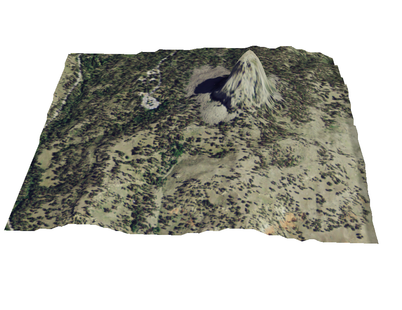
\includegraphics[width=4.0in]{FIGURES/tower1}}
 \caption[FDS file overview]{Devils tower }
\label{devilstower}%
\end{figure}


Devils Tower II

This example is similar to the first. It uses the -show command line option of dem2fds to add file names
to the terrain images and to show a red rectangle for the region being simulated.
This is useful for ensuring that the correct elevation and image files are being used and if not which ones should be downloaded.

dem2fds input file:
The longitude/latitude region is larger than in the first example.
It corresponds to the region of the data files that were downloaded rather than the region being modeled.

GRID
 100 100 30
LONGLATMINMAX
 -104.7256 -104.7096 44.5850 44.5945
create an fds input file using:
Again, the -show option is used to highlight the region being simulated and identify the files that were downloaded.

dem2fds -overlap -show -dir terrain/tower tower.in

where terrain/tower is a directory containing elevation data and terrain images for Devils Tower.

create the following image using the commands:
fds tower.fds
smokeview tower.fds

\begin{figure}[bph]
\centerline{
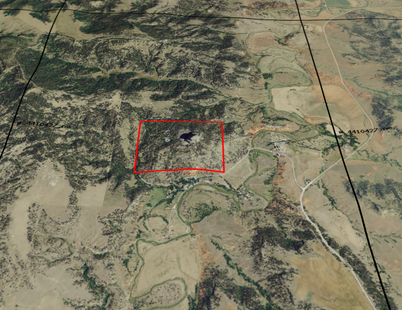
\includegraphics[width=4.0in]{FIGURES/tower2}}
 \caption[FDS file overview]{Devils tower }
\label{devilstowerB}%
\end{figure}

